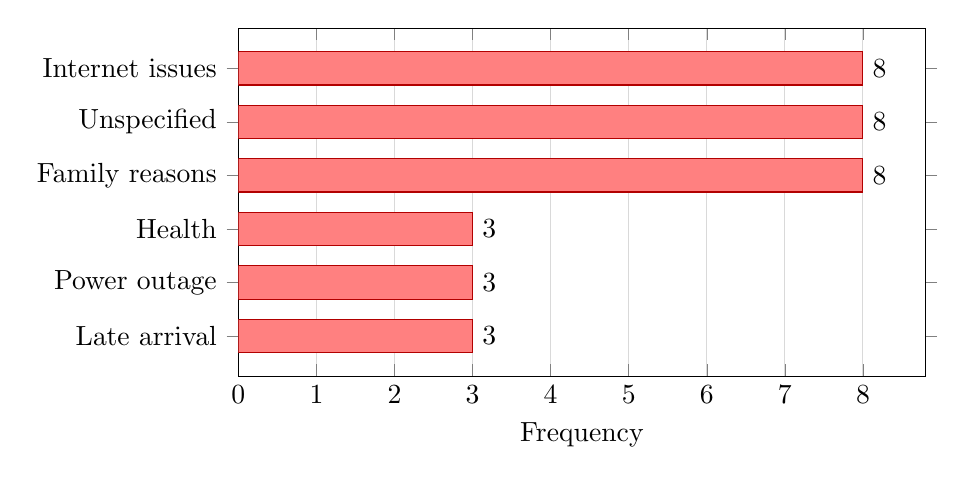
\begin{tikzpicture}
\begin{axis}[
    width=0.85\textwidth,
    height=6cm,
    xbar,
    xlabel={Frequency},
    symbolic y coords={{Late arrival}, {Power outage}, {Health}, {Family reasons}, {Unspecified}, {Internet issues}},
    ytick=data,
    nodes near coords,
    nodes near coords align={horizontal},
    bar width=12pt,
    xmin=0,
    enlarge y limits=0.15,
    xmajorgrids=true,
    ymajorgrids=false,
    grid style={gray!30},
]
\addplot[fill=red!50, draw=red!70!black] coordinates {(3,{Late arrival}) (3,{Power outage}) (3,{Health}) (8,{Family reasons}) (8,{Unspecified}) (8,{Internet issues})};
\end{axis}
\end{tikzpicture}